\documentclass[11pt,a4paper]{article}
\usepackage{a4wide}
\usepackage{amstext}
\usepackage{pdfpages}
%%\pagestyle{empty}

\begin{document}

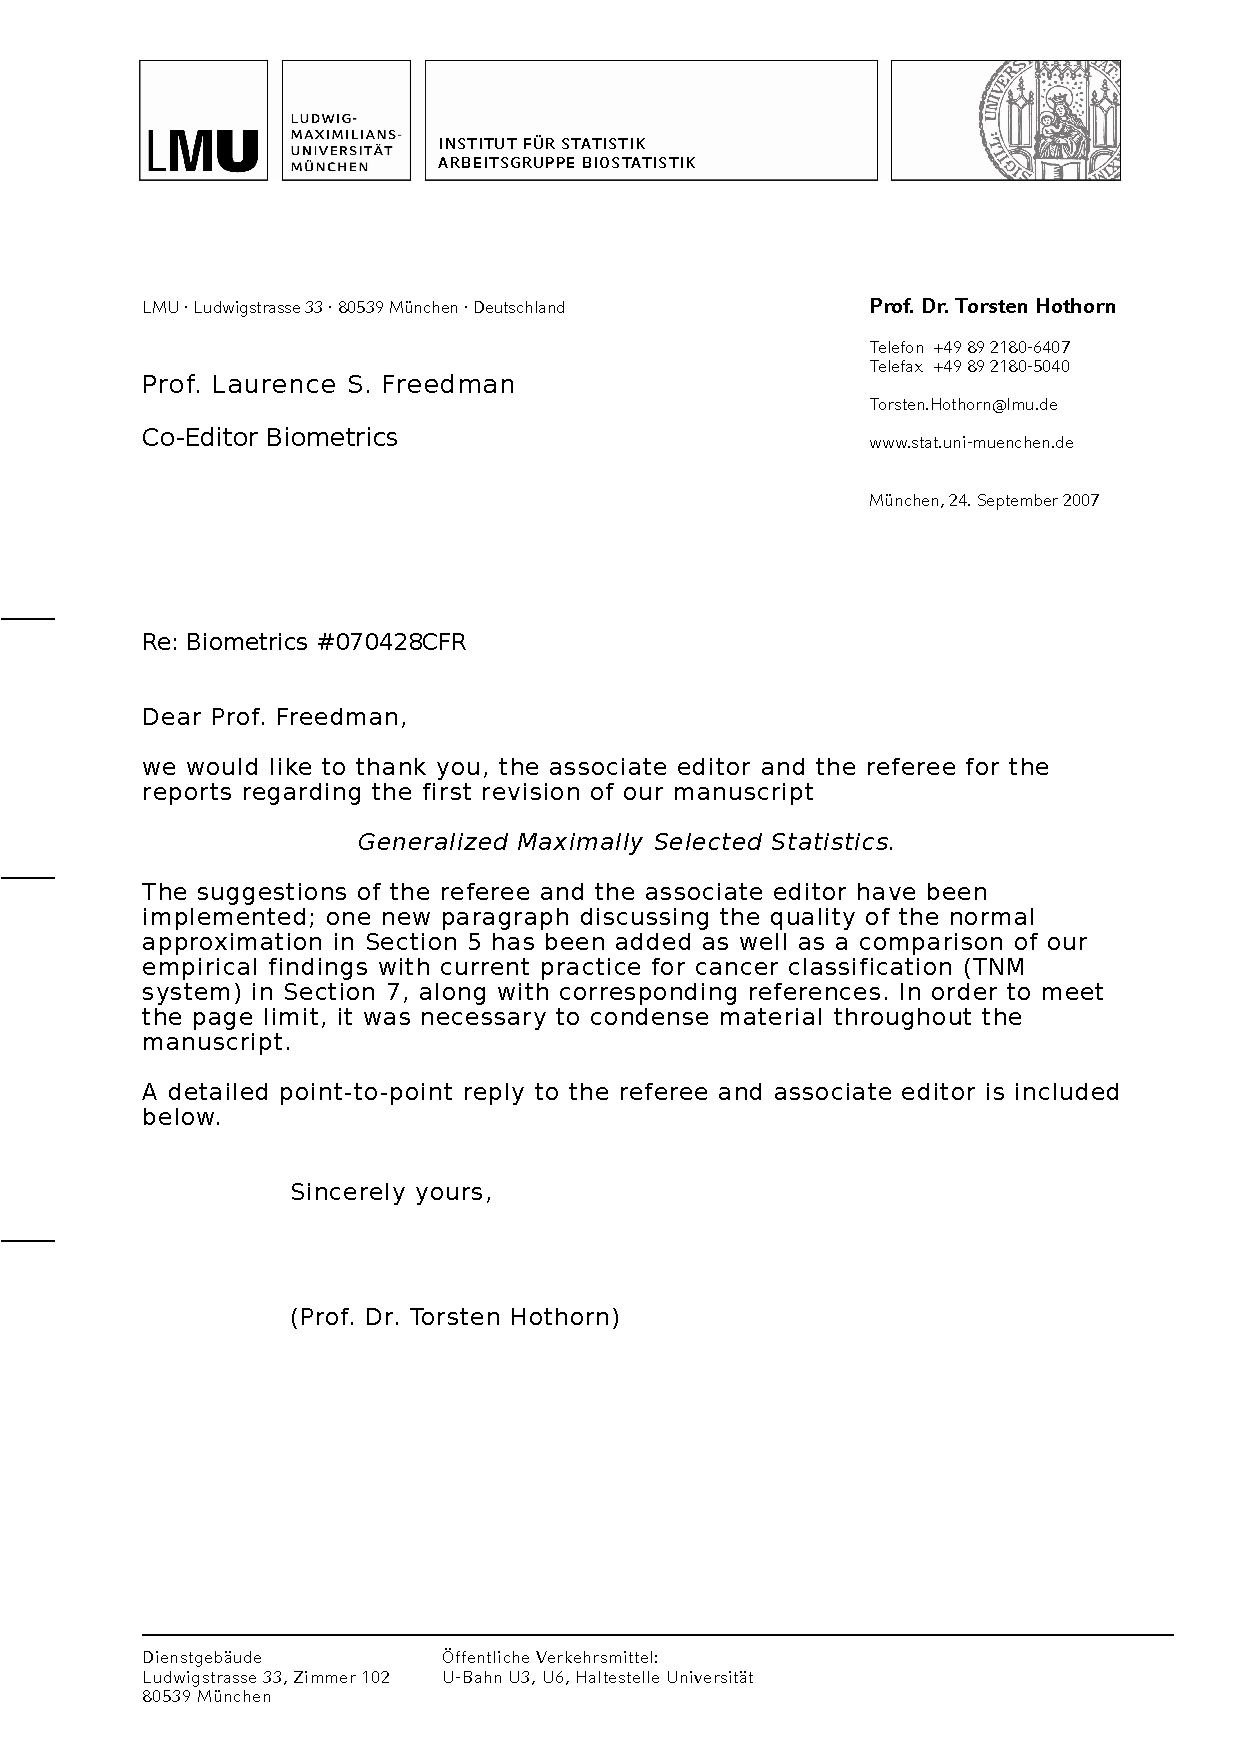
\includepdf[pages=1-]{biometrics2.pdf}

\begin{center}
\textbf{\large Point-to-Point Answers to Manuscript \#070428CFR \\
Generalized Maximally Selected Statistics} \\
by Torsten Hothorn and Achim Zeileis
\end{center}

\vspace*{1cm}

\textbf{\large Referee}

\begin{itemize}

  \item \textit{Please explain the connection between the novel procedure
for assessing interactions with maximally selected statistics and
the technical report available from: \\
http://www.statistik.lmu.de/~carolin/research/A-LB\_etal\_07.pdf}

The technical report derives the unconditional distribution of
a maximally selected $\chi^2$ statistic based on interactions
of nominal variables (SNPs, in this particular case). The idea 
can be implemented in an unconditional way as described in 
our manuscript and we added a reference to the technical report.

\item \textit{The article by Boulesteix and Strobl has now appeared:
Boulesteix and Strobl (2007). CSDA 51:6295-6306.}

Thank you very much for the hint, the reference has been updated.

\end{itemize}

\textbf{\large Associate Editor}

\begin{enumerate}

  \item \textit{The example needs to be embellished more given it's a Biometrics paper. One area of
embellishment would be to relate the thresholds to the clinical thresholds, as the authors
say in their response that the results are similar. This would lend clinical face validity
to the method.}

The results of our partitioning procedure, implementing simultaneous cutpoints 
in both T- and N-category, correspond rather closely to a prognostic factor study 
utilizing patients from the same trial. The reference has been added.

\item \textit{The authors’ response to item 4) of the previous AE comments provides a useful
example for ensuring a reasonable asymptotic approximation that would help the reader
implement the method. Accordingly, the authors’ should consider incorporating this
useful example on p. 9-10 by reducing the discussion of the theoretical discussion of
comparing approaches.}

A new paragraph has been added to the end of Section~5, discussing the
quality of the normal approximation for each of the elements of the
linear statistic $\mathbf{T}$.

\end{enumerate}

\end{document}
